% no answer key
\documentclass[letterpaper]{article}

\usepackage{units} 
\usepackage{parskip} 
\usepackage{xfrac} 
\usepackage[fleqn]{amsmath}
\usepackage{cancel}
\usepackage{float}
\usepackage{mdwlist}
\usepackage{booktabs}
\usepackage{cancel}
\usepackage{polynom}
\usepackage{caption}
\usepackage{fullpage}
\usepackage{comment}
\usepackage{enumerate}
\usepackage{graphicx}
\usepackage{mathtools} 
\usepackage{commath}
\usepackage{todonotes}

\everymath{\displaystyle}

\includecomment{note}

\title{Coins Flipping}
\date{\today}
\author{}

\begin{document}

  \maketitle
  % \listoftodos{}

  John Kerrich was a South African mathematician who spent WW II in a prison camp
  flipping coins.

  \begin{table}[H]
  \centering
    \begin{tabular}{rrrrr}
      \toprule
          & tosses & heads & difference & percentage \\
      \midrule
      1   & 10     & 4     & -1         & 40.00 \\
      2   & 20     & 10    & 0          & 50.00 \\
      3   & 30     & 17    & 2          & 56.67 \\
      4   & 40     & 21    & 1          & 52.50 \\
      5   & 50     & 25    & 0          & 50.00 \\
      6   & 60     & 29    & -1         & 48.33 \\
      7   & 70     & 32    & -3         & 45.71 \\
      8   & 80     & 35    & -5         & 43.75 \\
      9   & 90     & 40    & -5         & 44.44 \\
      10  & 100    & 44    & -6         & 44.00 \\
      11  & 200    & 98    & -2         & 49.00 \\
      12  & 300    & 146   & -4         & 48.67 \\
      13  & 400    & 199   & -1         & 49.75 \\
      14  & 500    & 255   & 5          & 51.00 \\
      15  & 600    & 312   & 12         & 52.00 \\
      16  & 700    & 368   & 18         & 52.57 \\
      17  & 800    & 413   & 13         & 51.62 \\
      18  & 900    & 458   & 8          & 50.89 \\
      19  & 1000   & 502   & 2          & 50.20 \\
      20  & 2000   & 1013  & 13         & 50.65 \\
      21  & 3000   & 1510  & 10         & 50.33 \\
      22  & 4000   & 2029  & 29         & 50.73 \\
      23  & 5000   & 2533  & 33         & 50.66 \\
      24  & 6000   & 3009  & 9          & 50.15 \\
      25  & 7000   & 3516  & 16         & 50.23 \\
      26  & 8000   & 4034  & 34         & 50.42 \\
      27  & 9000   & 4538  & 38         & 50.42 \\
      28  & 10000  & 5067  & 67         & 50.67 \\
      \bottomrule
    \end{tabular}\caption{Coin flip data.}
  \end{table}

  \begin{figure}[H]
    \centering
    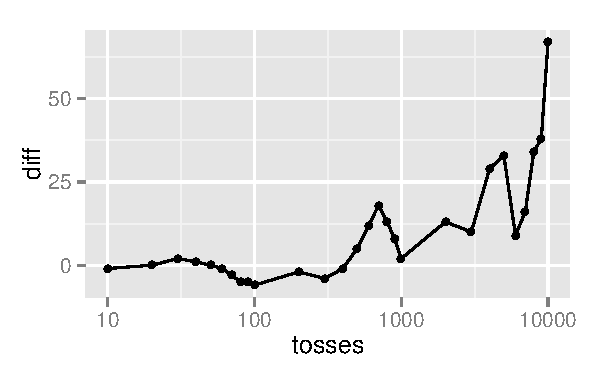
\includegraphics[scale = 1.3]{figures/diff.pdf}
    \caption{Difference from expected}\label{fig:diff}
  \end{figure}

  \begin{figure}[H]
    \centering
    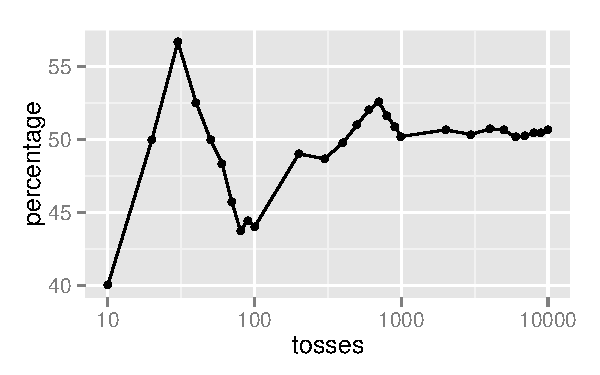
\includegraphics[scale = 1.3]{figures/percentage.pdf}
    \caption{Percentage heads}\label{fig:percentage}
  \end{figure}


\end{document}

